\section{Model framework: introduction \label{sec:frameworkintro}}

This chapter has two aims:

\begin{itemize}
	\item Explain how model `scenarios' are coded, described and presented
	\item Explain the logical structure of the model framework
\end{itemize}

The main goal of the model framework is to provide methods for easily comparing different spatial economic scenarios. To do this, it needs to be able to deal with a large number of different options. The range of these options is potentially confusing; this chapter aims to reduce that confusion to a minimum by clearly laying out a reference guide to the available options. It also explains how a particular option-set (a `scenario') is described when model results are presented.

The model framework implements the key economic and space concepts from chapter \ref{chapter:location} and provides a structure for agents using them to interact. It is built using object-oriented programming, as discussed in section \ref{sec:OOP}. Relations between objects can be used the describe the logic of the model if they are divested of unnecessary detail. Table \ref{tab:keytable} gives a key for the diagrams that will be used to do this. (Appendix \ref{apx:modelcodeoverview} describes the code more traditionally, using UML.) The rationale for this approach is to present the object structure and the logic of the algorithms in one diagram as clearly as possible, but they should be used in conjunction with the text description. One coding norm that will be used here is to capitalise objects, when they are being discussed as objects. For instance, `Good' is a particular object, distinct from goods generally. 

\subsection{Chapter overview}

The chapter covers the following topics:

\begin{itemize}
	\item The next section describes the three elements that form the foundation for the model framework: actor setup, decision structure and actor data - these are outlined briefly and then discussed in more detail below
	\item The units used in the model are explained
	\item The next section describes Actor setup for Firms and People in detail
	\item The model `scenario' description method is outlined
	\item The chapter ends with a discussion and critique
\end{itemize}

\cmt{and may end with checking the basic economics, though that might go into the next chapter}

\input{ChapterFramework/Tables/keyTable}

\section{Elements of the model \label{sec:elementsmodel}}

\subsection{Two actor setups \label{sec:frameworkActorSetup}}

The two actor setups are:

\begin{itemize}
	\item Single actor type only
	\item Two actor types: People and Firms
\end{itemize}

The single actor setup requires all actors to decide who else to interact with. No exogenous distinction between Firms and People is built into the model structure. Two-type models, however, do impose that distinction: Firms and People have separate decision structures and motivations. 
\cmt{This draft sticks with explaining the People-Firm model. I'll need to explain the single actor version somewhere. I'm getting the most complex one done first before worrying about that.}

\subsection{Decision structures and model timeline \label{sec:frameworkDecisionStructures}}

\begin{figure}%
\centering
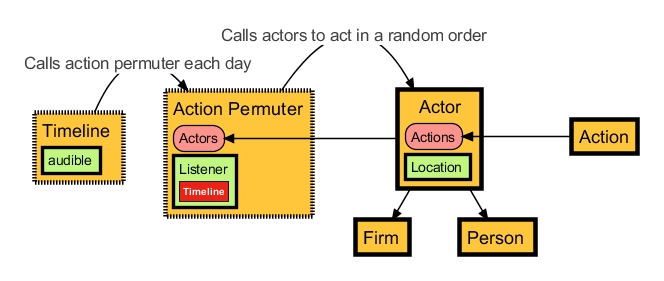
\includegraphics[width=0.75\columnwidth]{ChapterFramework/figures/TimelineActions}%
%\includegraphics[width=0.85\columnwidth]{ChapterModels/Figures/hillclimbExcel}%
\caption{Timeline sequence}%
\label{fig:frameworkTimeline}%
\end{figure}

The timing structure shown in figure \ref{fig:frameworkTimeline} is very simple: as each day passes on the `Timeline', an `Action Permuter' calls all actors in a random order.\footnote{The Timeline is part of an Observer framework used by other model elements like visualisation and data writing; again, see the code appendix for more details.} When an Actor is called, they decide what action to take. Actors' decisions are based on one or both of the following:

\begin{itemize}
	\item Instant: act on information collected `now'
	\item Feedback: Act, wait, respond
\end{itemize}

As discussed in section \ref{sec:blindvsrational}, actors take decisions either instantaneously or using feedback from their actions over one or more timesteps. In instant decisions, when actors are called to act, they immediately gather the information they need and optimise based on that. For multi-timestep decisions, actors try an action and then check later whether the outcome was desirable or not before taking their next action. No attempt is made to simulate synchronous decision-making. At the point where an actor is deciding, all others are currently static.
\cmt{more on async vs sync decision-making}
\cmt{Separation of timings for different agent types. Needs covering. Here?} 

%Types of actor decision structure to describe: backyard, firm + people, with people taking instant decisions, firms multi-timestep.
\subsection{Two actor data sources}

Actor decisions will be based on one or both of the following sources of information:

\begin{itemize}
	\item Internal actor data, changed by other actors since last a decision was taken. (Example: firm net income.)
	\item Externally collected data (Example: list of good prices from surrounding firms.)
\end{itemize}

Externally collected data can come only from other Actors. This is acquired by searching space for a list of all appropriate Actors and forming a set from it.

These three elements - Actor setup, decision structure and Actor data - form the foundation for the model framework. Section \ref{sec:actorSetup} explains how they are put together. Because all actors face a static world at the point where they decide, their actions can be logically described separately.

%%%%%%%%%%%%%%
% UNITS
%%%%%%%%%%%%%
\section{Model units \label{sec:modelunits}}

\subsection{Use of space }


%I cut out the descriptions for the space chapter - where they came from to start with!
The size of both $R^1$ and $R^2$ is kept to one number: in $R^2$, width and height are always kept the same. 

Model space is measured in very small units. If space is not wrapped and there is no reason to examine overlapping actor interaction, a width of one is usually used, since it keeps things as simple as possible. If space wraps (either a `racetrack' or torus world), it must be large enough to make sure actors' spatial search does not overlap itself. For example, if an actor can travel for `one day', their full search circumference spans two days, and the size of the space they are in must be at least this large. In some model runs, the distance actors can reach in one day is increased. In these cases, world dimensions are defined so that the maximum reach keeps within the boundaries just described for either wrapped or discontinuous space.
\cmt{where am I discussing normalising a `day' to space? And do I need a diagram to explain this?}

This choice of spatial measurement impacts on how space costs must be set. Many of the models use a `delivery cost' for goods (see section x below for full details.) In a world that is only one or two units wide, and where actors may be clustered together in a small part of that space, good movement costs must be proportionately higher to have any economic impact.
%Probably need to explain how it affects discrete outcomes somewhere

%In the models that use explicit space, distance measurement is built around the idea of one Person's `day'. The distance a Person can get in one day serves as one unit. That distance Actors can get in one day may change over a model run, but it still stands as a base for comparison in that run. Distances will be described this way:

%Moved to space costs chapter

%As discussed in section \ref{sec:spacechange}, any factor that can be used to `buy movement' will be labelled an \gls{mbf}: units of distance can be bought with it. Depending on the type of actor, specific \gls{mbf}s \emph{must} be spent to cover distance. The most obvious \gls{mbf} is time: it takes a certain quantity of time to cover a given distance. For the sake of readability, `units of distance' will be referred to as `miles': these are entirely abstract, and are used purely to make description more readable (`miles per day' rather than `distance units per day'.) A factor can be an \gls{mbf} as well as a standard productive factor entering into a firm's production function. Again, time fits this description: where People are not putting time into moving, they can put it into production. Often, economic models use the term `labour' to refer to this productive factor; in the core model, it is the only factor. In more detail:

%\begin{itemize}
%\item For each model day, each actor is given $t=1$ to spend: in other words, they have `one day per day' and will aim to make optimum use of it. (See note below for more on this.)
%\item A given distance between $r$ and $s$ will be labelled $rs$. The time is takes to cover it is $t_{rs}$. So, generically, $t_{rs}=f(rs,tech)$, where $tech$ is some technology that has an impact on the time taken. For many of the models, time to cover a given distance will be a function of the distance alone. However, the generic factor $tech$ here indicates that the amount of time to cover a distance may change. 
%\item $tech$'s role in this function is separate from its cost. For example, if $t{}_{rs}=rs/tech$, the time taken to travel between $r$ and $s$ goes down as the level of $tech$ increases. It says nothing about $tech$'s cost. Indeed, from the point of view of actors, it could be free and ubiquitous.
%\end{itemize}

%q: what's the average distance between randomised actors in a one-width world? Well: of course, it drops as more actors are added. Oooh - that's interesting! Didn't think of that before! If I want to control distance between actors, that needs fixing!

%What other values do I need to discuss? How to measure changes in clustering, thus agglomeration. What units? And for good movement cost, which we'll call delivery cost. Actually, I'm not sure how I've defined that! It has to be large because of the small size of the world, of course, if it's to have an impact.
%Then there's: wages, good price etc.

%%%%%%%%%%%%%%%%%%%%%%%%%%%%%%%%%%%%
% MODEL VARIABLES AND NORMALISIN' EM
%%%%%%%%%%%%%%%%%%%%%%%%%%%%%%%%%%%%
\subsection{Model variables and keeping them normalised in an abstract setting}

The model framework is abstract: the purpose of specific values for variables, then, is always relative to other values in the model itself, not any external quantity. Because of this, it is always best as far as possible to normalise the values used in order to keep the analysis as simple and clear as possible. Where appropriate, this will mean just using unity (a value of one). This section describes the values used, explains how they are normalised, and how they will appear in the model data presentation.

\subsubsection{Economic variables}

For 'Firm and People' models, the two key economic variables are wage and good price. These both need setting in proportion to each other, as the real wage is actually purchasing power, not the nominal model value. (As discussed below, however, the real yardstick for the model is the amount of utility actors can get for their time.) This is most obvious when using the Engel function as People's utility: the price ratio of wage to goods will determine whether any demand exists for the luxury good. For example, if $\gamma=1$, and wages and goods are both one, only necessity goods will be demanded (with some tiny quanity of random luxury buying - see below.) If wages are twice as high as basic good prices, however, demand for luxury goods will kick in. Since it is this ratio that is key, not the nominal value, model wage values will always start at one and other values changed if necessary.
\cmt{Using 'utility for time' as yardstick: where else have I discussed this? This section needs a re-order... Also, I'm saying here the two key economic vars are wage and good price: not so in single-actor models. }

\subsection{Space costs 1: good cost method...\label{sec:spacecost1}}

The total price of a good includes the cost of moving it across space. Consider a good $g$. The total price is $P_g$, and consists of three parts: $p_g$, the base price; $c$, the cost to move one unit of the good across one unit of distance; and $d$, the distance itself. So in full:

\begin{equation}
P_g = p_g + (c \cdot d)
\label{eq:totalgoodcost}
\end{equation}

If $c = 0$, then, the good will cost the same anywhere in space. If $d = 0$, a Person is at the same location that the good is being sold from and, again, only has to pay the base price $p_g$. The variable $c$ is the simplest way possible to represent the cost of moving goods across space. The fact that it is the cost per unit of distance means it can stand in for weight. Section \ref{sec:explorechangingcosts} works through the mathematical implications of this.


%at least, the current good cost method
%%%%%%%%%%%%%%%%%%%%%%%%%%%
% This is where Units started before...
%

%The thesis models are abstract: they are not calibrated to any particular real-world situation. As far as possible, then, values are normalised to keep analysis and presentation as clear as possible. That said, it is still worth discussing the way numbers are set up in the model.

%In defining parameters, some concepts from object-oriented programming are borrowed. Variable parameters can vary at any time in or between model runs. Static parameters are fixed for single model runs, but may vary between runs if, for instance, they are subject to a parameter sweep or randomisation. Final parameters never change. Where appropriate, a description will also be given of the exact way in which parameters change. Most commonly, this will be whether wages, prices, stock and money are fixed and if not, how they are set. 
\subsubsection{bits}

Some values represent excludable, rivalrous values, where only one actor can `have' them. Both stock and money can come into this category, but note that in a particular model `scenario' (see below), the `flow' of these values may be turned off. For example, if the wage and goods prices are both fixed, money flow may also be turned off.

%\subsubsection{Space units}

Since each Person has one day to spend, the number of People determines the total amount of available labour in any model scenario. If People are also spending that day on movement, there is thus a zero-sum relationship between time contributed to production versus space.

Lastly, the nominal value of wage and good price matters less than their ratio: what a Person can buy with their wage. This is the `real wage'. 

%%%%%%%%%%%%%%%%%%%%%%%%%%
% ACTOR SETUP
%%%%%%%%%%%%%%%%%%%%%%%%%%
\section{Actor setup \label{sec:actorSetup}}

%%%%%%%%%%%%%%%%%%%%%%%%%%
% PERSON
%%%%%%%%%%%%%%%%%%%%%%%%%%
\subsection{How People act \label{sec:howPeopleAct}}

\begin{figure}%
\centering
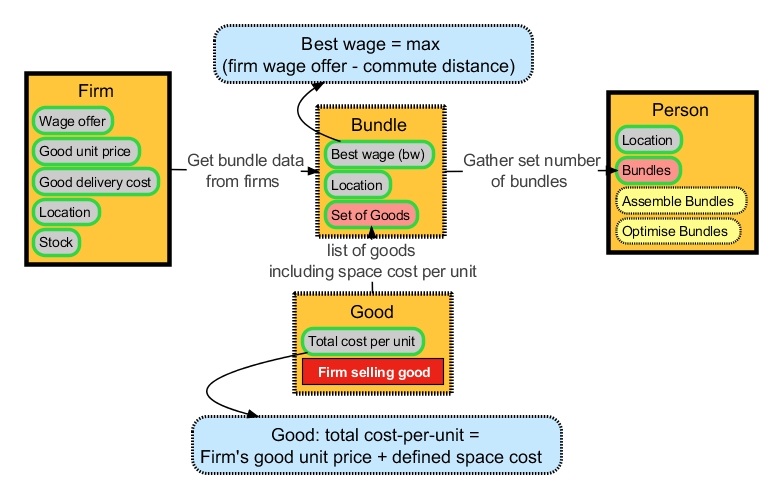
\includegraphics[width=0.95\columnwidth]{ChapterFramework/figures/PersonAction1}%
%\includegraphics[width=0.85\columnwidth]{ChapterModels/Figures/hillclimbExcel}%
\caption{Elements for the Person action}%
\label{fig:personlogic1}%
\end{figure}

%\subsection{How do People turn time into utility? \label{sec:turntimetoutil}}
People have `one day per day' to spend and, as section \ref{sec:keyconcepts_coremodel} pointed out, their fundamental question is, `what is the maximum utility I can get for my time?' This time can be spent on moving through space, on production in their own backyard, or put into firms or collaborators in exchange for either goods or money. The description here deals with the most complex of these: people working for money and then spending it on goods. 

People compare a number of `Bundles'. Each Bundle consists of a location, a best wage offer and a list of goods. They then choose the one that will give them the highest utility. 

%How exactly does this happen? There are two elements:
%\begin{itemize}
%	\item Bundles are assembled.
%	\item Bundles are optimised to turn People's time into the best possible utility.
%\end{itemize}

Figures \ref{fig:personlogic1} and \ref{fig:personopt1} outline what happens when a Person is called to act. An `instant' decision is made on what to buy, who to work for and where to locate based on data they gather when it is their turn. Figure \ref{fig:personlogic1} shows all the elements prior to utility maximisation. As well as their set of Bundles, People have two methods: `assemble Bundles' and `optimise Bundles'. The next section (and figure \ref{fig:personopt1}) describe this last step in more detail. An overview of the methods involved is as follows: 
%\cmt{in a situation where there are firms. How/where to describe other scenarios? Get this one done first, then think about it.} 

\begin{itemize}
	\item Method `assemble Bundles': assemble a series of Bundles; one from my current location, and a defined number from other random locations.
%	 A single Bundle is put together as follows:		
\item Method `optimise Bundles': two steps. 
\begin{itemize}
	\item Optimise each bundle's mix of goods to get a single utility value
	\item Select the Bundle with the best utility: accept the wage, pay for goods and, if applicable, move to the new location.
\end{itemize}
\end{itemize}

%\begin{itemize}
%	\item Get bundle data from Firms: gather a list of Firms, either within a given distance range, or for the whole model space. This gives access to the necessary firm data: the wage offer, good unit price, delivery cost and location.
%	\item From that list, keep a record of all goods: their total cost per unit, including any delivery costs; the available stock; which firm is selling
%	\item Also keep a record of the firm offering the best wage, accounting for commute distance. 
%\end{itemize}

\subsubsection{Assembling Bundles}

As outlined in figure \ref{fig:personlogic1}, a Bundle consists of the following: 

\begin{itemize}
	\item The centre location of the Bundle. One of these will centre on the Person's current location. Others are given random locations within a defined range. The rationale here is this: each separate Bundle allows a Person to ask, `if I were to move to that spot, would I get a better utility value?'
	\item A set of Goods, where each Good is an object containing the good's total cost per unit (including delivery cost) and a reference to the Firm selling the good. That reference provides a way to check stock levels as well as to buy goods from Firms if the Bundle is selected.
	\item A `best wage' selected from a set of Firms and taking account of commute cost.
\end{itemize}

Each of these is dealt with next, but here are a few preliminaries. Firstly, What determines the number of random bundles? The value is arbitrary: the higher it is, the more likely on any one turn that a person will find the `best' utility option for them. Over a number of days, however, this will tend to happen anyway. Section \cmt{Section on sensitivity testing for timing structures} goes into the issue in more depth: what difference do timing structures make for outcomes? The range for a Bundle's centre location can also vary. It may be limited by one day's distance, weighted towards closer distances, or People may be given free choice over the whole model space.

The first step for a person getting Bundle data is to get two lists of Firms: one for finding the best wage, another for a full list of available goods. Two sets are required since distance to potential employers may be restricted by commute distance, whereas good delivery can occur from further afield.

\subsubsection{Getting a set of Goods} 

A Bundle will contain a list of all goods, either within a given range or for the whole model space. Each good is represented by a `Good' object that contains the following:

\begin{itemize}
	\item Cost per unit, including delivery cost.  
	\item Reference to the Firm selling the good.
\end{itemize}

As regards good delivery costs, there are various ways of calculating this. See section x \cmt{Section for outlining approaches to pricing goods across space} for full details, but an example illustrates the principle. If a firm has a base unit price $p$ and a delivery cost to move one unit for one `mile' $d_{p}$, and the distance to deliver is $af$, then the cost per unit can be set to $p + (p\cdot d_{p}\cdot af)$. This is the value stored in the Good object. The fact that a space cost is part of that is hidden to the Person: they make their decision based entirely on this single calculated cost.

\subsubsection{Selecting the best wage \label{sec:wageselect}}

\cmt{What I'd like to do here: use the set of Firm objects, and be allowed to define values within those objects, such as the firm wage offer, and location, so I can use one set notation line for saying what I mean. Options? Anyway - here's my attempt. If we go with this, I'll need to outline it above.}
\cmt{Also: zero sum time for commute or work - this is a movement-buying factor. Again, though, I'm just writing up the model as it stands and will work out where to put the MBF stuff (if at all) later.}

Each Bundle has one unique `best wage' offer. Selecting this is a two-step process: first, gather a set of all Firms within commute distance. Second, select the Firm offering the best wage, accounting for commute distance from the Bundle's location centre. This best wage can be described as follows. Let $F=\{f_{1},f_{2},...,f_{n}\}$ be the set of Firm objects. Each Firm has a wage offer, which is `the amount paid for one day's input'. For each $f\in F$, $W_{f}$ is that wage offer. To describe space cost, the distance in \emph{time} can be used: for each $f\in F$, $t_{fa}$ is the time taken to travel between $f$ and $a$. 

Let $l_{af}$ be the labour available to contribute to $f$ by Person $a$. The amount of labour they have available for contributing is just their own time (one day, $t_{a}=1$) minus commute time. Here, a `commute' is taken to be twice $t_{af}$. The upper distance limit on whether a firm enters into $a$'s considerations has to be less than $a$'s one available day in total - half a day there, half back - otherwise there is no time left at all to contribute to production. So $f$ can only be a maximum of half a day away. Given all this -

\[
l_{af}=t_{a}-2\cdot t_{af},\; 0<l_{a}<1\]

If $W_f$ is $f$'s wage for a full day, and $a$ has $l_{af}$ to contribute (a fraction of their full day), this means the wage they will get is just $W_{f}\cdot l_{af}$. The best wage for Person $p$ can now be defined as:

\begin{equation}
bw_p=max\; \{W_{f}\cdot l_{af}\mid W_{f}\in F,\; t_{af}<0.5\}\label{eq:bwpmax}
\end{equation}

So, the best wage for Person $a$ is the maximum value from the following set: all wage offers proportionate to Person $a$'s labour input from those firms in $F$ who are less than half a day away.

\cmt{Now, was that overkill? Could I just have used this last sentence?}

%%%%%%%%%%%%%%%%%%%%%%%%%%
% The optimisation routine
%%%%%%%%%%%%%%%%%%%%%%%%%%
\subsubsection{Optimising bundles \label{sec:optimisingbundles}}

Once a Bundle is assembled, it can be passed to the Person's optimisation routine.\footnote{As appendix \ref{apx:modelcodeoverview} explains, there is only one actual, static Optimiser class, but in terms of `functional isomorphism' it can be considered internal to each Person.} This produces a utility level, which is stored in the Bundle. Finally, the Bundle with the maximum utility level is selected: the wage offer is accepted and the optimal quantity of goods is bought.

%Section \ref{sec:frameworkUtility} goes into the full details of how this happens.
The logical goal is simple: for each Bundle, find out how to spend the best wage on the set of Goods as optimally as possible (without actually spending it) then choose the optimal Bundle. Figure \ref{fig:personopt1} is an overview of the process. Assuming the Person has the set of Bundles they will optimise, the sequence is as follows. 

\begin{figure}%
\centering
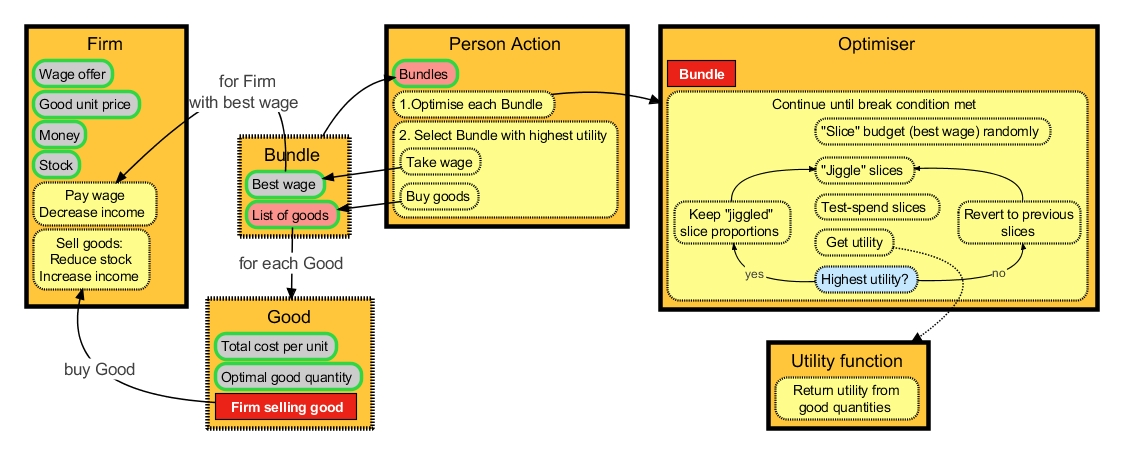
\includegraphics[width=1\columnwidth]{ChapterFramework/figures/PersonOpt}%
%\includegraphics[width=0.85\columnwidth]{ChapterModels/Figures/hillclimbExcel}%
\caption{Optimisation of Bundles in a Person's action}%
\label{fig:personopt1}%
\end{figure}

\begin{itemize}
	\item Optimise each Bundle. This happens in an Optimiser:
	\begin{itemize}
	\item The Optimiser iterates, either for a set number or until some condition is met (such as no marginal utility gain for a certain number of steps: see below.) 
	\item The iteration is initialised by randomly slicing the budget (the best wage), one slice for each Good in the bundle, before beginning the iterations. The iterations are:
	\item `Jiggle' the slices, changing their proportionate size slightly.
	\item `Test-spend' those slices on each Good: find out how much could be bought with the current budget slices using the per-unit price for the Good.
	\item Get a utility level for these quantities of goods. The Utility function is logically separate: the Optimiser deals only with this process of random slicing and adjusting.
	\item If the utility level found is the highest so far, keep the current proportion of slices and return to the 'jiggle' point. Else, revert to the previous slice proportions and try again. This has the effect of ratchetting the budget slices (and thus the spend per Good) towards an optimum.
	\end{itemize}
	\item Once each Bundle has an optimum utility, select the Bundle with the highest:
	\begin{itemize}
	\item Take the best wage: this instructs the Firm to pay the Person.
	\item Buy goods in the quantities found optimal by this Bundle.
	\end{itemize}
\end{itemize}

Figure \ref{fig:CESHillClimbIllustration} graphs data from this process in action. A bundle containing sixteen goods of equal cost is optimised for a CES function over a thousand iterations. (The optimum for a CES function with equal-value goods is  already known from section \ref{sec:CESbasics}: an even mix.) In this example, the optimum is found quite slowly: this helps to illustrate the process. The first graph shows initially random budget split guesses converging on the optimum mix of $0.06$ for each good. The second shows the marginal utility gain from each iteration; most of the gains happen very quickly, after which almost no extra benefit accrues (though there is a very small amount of further convergence.)

The important difference to analytic constrained optimisation is that people can work with any number and type of good and can deal with limited stock levels.
\cmt{Need to illustrate what happens in limited stock situations, what happens to money if it can't all be spent.}
In contrast, a standard constrained optimisation results in an `objective' optimum (see \ref{sec:produtility_agents}). In this model framework, people may find that this optimal amount simply isn't available to them, so they must spend their wage accordingly. As well as being able to deal with any quantity of available good, this approach also allows easy swapping of utility functions: there is no need to produce separate constrained optimisation equations for different situations.

\cmt{somewhere: need to compare this limited notion of rationality with the critiqued `superhuman' rationality that conflates the ability to tell better from worse with perfect knowledge of the whole market. Also, the `realism' of 1000 iterations for finding utility. Here probably isn't the place. Also x-ref to Fowler's agent model, which uses objective optima, and Firms can use that signal.}

\begin{figure}%
\centering
\includegraphics[width=0.85\columnwidth]{ChapterModels/Figures/hillclimbExcel}%
\caption{Utility-maximising stochastic search algorithm, optimising a CES function with 16 goods over a thousand iterations (x axis)}%
\label{fig:CESHillClimbIllustration}%
\end{figure}

%%%%%%%%%%%%%%%%%%%
% UTILITY
%%%%%%%%%%%%%%%%%%%
\subsubsection{Overview of People's utility \label{sec:frameworkUtility}}

%Things to do here:
%Give a run-down of the actual utility details and how it fits together
%Give a run-down of the structure of the optimisation

The technical detail of optimising utility has just been covered. There are three further points worth covering briefly.

People have utility functions based on those described in section \ref{sec:econconceptsintro}. In any one model run, all actors have identical tastes: they all use the same utility function. One useful assumption from using identical tastes is that, in one-good models, only the absolute quantity of that good matters. This is because the same quantity of good will always return the same utility for each Person, regardless of the form of utility. For example, if all people have an identical one-good utility function that happens to have increasing returns, the increasing returns will just produce the same level of utility for everyone, given the same good input. In contrast, if tastes were not identical, one Person could gain more utility from the same quantity of good as another. Section \ref{sec:backyard} discusses a one-good situation where the raw-good amount stands in for utility.

In all situations where more than one good is available, People use utility functions. The form of utility used must also imply the production structure, though not the actual production function itself. For instance, a two-good utility function means a model where only two goods are made, though many firms may compete to sell each good. An $n$-good utility scenario, using the \gls{ces} function, will have each firm making one unique good, as they do in \gls{monocomp} models.

Actors using this method are rational in only the most basic way: they are able to judge when one Bundle is better than another. This rationality reflects basic micro-economic preference assumptions. Bundles of goods are `complete': any two bundles can be compared. They are also transitive: as Varian puts it, ``if the consumer thinks that $X$ is at least as good as $Y$ and that $Y$ is at least as good as Z, then the consumer thinks that X is at least as good as Z'' (\citealt{varian_intermediate_2006} p.35). 

%Why take this approach, when it is possible to produce constrained optima that include price? 
%MM1 20pp/23	Reasoning behind bundle approach; cf. to Fowler's 'objective demand' approach. Write up.

%again, I'm not sure where to discuss the hill-climb, the black-box nature of it, compared to some `online' approach. At the moment, I haven't used the online approach, so I'll leave it. Needs discussing somewhere.

%%%%%%%%%%%%%%%%%%%%%%%%%%%%%%%%%%%%%%%%%%%%%%%%%%%%%%%%%%
% HOW FIRMS ACT
%%%%%%%%%%%%%%%%%%%%%%%%%%%%%%%%%%%%%%%%%%%%%%%%%%%%%%%%%%
\subsection{How Firms act \label{sec:howFirmsAct}}

A Firm's decision process is based on feedback between timesteps. A firm takes an action, waits, and then responds depending on how its own internal data has changed (see figure \ref{fig:FirmAct1}). Because of this, the structure of Firm decision-making is quite a lot easier to describe, since Firms do not collect any data externally themselves. 
\cmt{At least in the simplest version they don't. They might at some point: may be the only way to solve coordination?}
At time $t-1$, a firm chooses one of either location, good unit cost or wage offer, and `jiggles' it, altering it slightly in a random direction. It remembers these choices. At time $t$ the firm asks, `did my net income between timesteps increase?' If yes, it repeats the previous action (hence needing to remember what it was), with the possible addition of increasing the size of the adjustment. If not, the Firm returns to its initial random search.
\cmt{again: this is their current method. Given I want to address coordination, this will be added to. Has been already, but needs more work.}

\begin{figure}%
\centering
\includegraphics[width=0.85\columnwidth]{ChapterFramework/Figures/FirmAct1}%
\caption{A Firm's feedback mechanism: ``jiggle'' a random value, wait to see effect.}%
\label{fig:FirmAct1}%
\end{figure}

The result is that, through blind search, Firms are constantly searching for ways to improve their net income. Note that this method disconnects them even further from any analytic approach to optimising. Where at least People do use a utility function (albeit one that calculates utility solely from raw good amounts), here the firm does not directly consider its own input or output requirements. Also, while they act on how their own internal data changes, Firms know nothing about how those changes occur. 
\cmt{and this is a key area where I need to work through other options that might help the firm coordinate better.}

\subsubsection{Firms' production functions}

The simplest Firm production function turns a given amount of labour input into good output. For a given time period, how can this be worked out? Section \ref{sec:dmr} explored the problems of getting agents to utilise increasing returns in an agent-based time structure. The goal is to allow the model's Firms to gain from those increasing returns: output per unit of input labour should increase as the total labour contribution rises. The problem is finding an effective way to allow that total labour quantity to change, given the discrete, asynchronous nature of decision-making.

The solution used is as follows. Two things happen: first, when a Person chooses an employer, they receive their wage on the spot, and their contribution to the Firm's production is calculated then and there. However, they `leave' a record of their contributed time with their chosen employer until it is their turn to act again, when they remove it and decide anew. This means that, when anyone else comes to contribute, that time is still considered as an input, as far as the production function is concerned. This allows increasing returns to occur. This approach is discussed in more depth in section \ref{sec:backyard} to see exactly what impact its assumptions have on model outcome.

%%%%%%%%%%%%%%%%%%%%%%%%
% SINGLE ACTOR MODELS
%%%%%%%%%%%%%%%%%%%%%%%%
\section{How the single-actor models work \label{sec:singleactorFramework}}

Using a single actor-type does away with many of the complications that come with modelling the interaction between Firms and People. Most importantly, single `Actors' need only seek to directly improve the utility they can get for their time. There is no intermediate stage where money is required for wages or good purchase.

In these scenarios, Actors always have the option of simply producing in their backyard. This gives a base for comparison: one day's input will always return one unit of utility. For anything spatially interesting to happen, then, Actors must be able to find outcomes that can better this backyard situation: utility must be more than one.

Section x outlined what this means: there must be a form of increasing returns. Without this, any space cost guarantees that backyard production will always be the better option. There two two forms of increasing returns, and either can give Actors the ability to find better-than-backyard options: economies of scale and love of variety.

\cmt{here I need to carefully lay out if/when there are any differences between LoV and EoS as far as agent choice goes, and what the space cost implications are. In some respects, they're no different...}

On the face of it, \gls{eos} and \gls{lov} produce higher utility in very different ways. \gls{eos} stem from a more-than-linear increase in output for a given input into production, whereas \gls{lov} is a purely utility-based function. Mathematically, however, output from both \emph{can} appear identical. \gls{eos} does not need to be a physical output increase; it can be an increase in the value of each unit. If this was the case, physical weight per unit of value (value density) could increase \emph{or} decrease.

Another difference, one might argue, is that \gls{eos} implies an indivisibility. In the case of labour, workers must come together at a particular site to produce the goods. Again, however, \gls{lov} can be said to require the same: there must be a `point of trade' for the exchange of goods and, even if they are not consumed at that point, the future utility-increasing consumption is implied in the exchange's successful outcome - otherwise it would not have taken place.



Aside from that, the output could be physically less, physically more. Generally it would need to be worth more to be economically feasible, but that doesn't logically have to be the case: people could be coating electronics in marmite, thus ruining it and making it heavier.
Looking at LoV, the same outcome occurs - pretty much:
Point of trade is where the increasing returns are
No extra physical output, pure increase in value. Pretty much costless: value comes about purely through exchange. Cheapest value creation possible. (Though not free since it needs to be got to market.)



%%%%%%%%%%%%%%%%%%%%%%%%
% MODEL SCENARIOS
%%%%%%%%%%%%%%%%%%%%%%%%
\section{Model `scenario' setup \label{sec:scenarioFramework}}

Individual model `scenarios' will examine a particular aspect of the thesis issues. For each scenario, the main components will be described in table form as succinctly as possible. Where a scenario has particular idiosyncracies, these will be described below the model scenario table. 

\subsection{Model scenario description method}

The \emph{components} of model scenarios vary in a limited number of ways: table \ref{tab:components} lists these commonalities, and the following discussion explains the table entries in detail. 
%Following this, model \emph{parameters} will also be outlined. 

\input{ChapterModels/Tables/modelComponentsTable}

\subsubsection{Run type}

Model iterations are considered `days'. A model run will last a set number of days. Generally, all actors will take an action at least once a day (with some exceptions where firms only respond every few days.) The particular number of days chosen will vary depending on the appropriate amount of time needed to find a useful result. 

In each scenario, a single model run will be used to illustrate the basic point. Subsequently, parameter sweep runs may be used. These repeat model runs, while altering a particular parameter. See the discussion of parameters below for a consistent way of describing how they change.

\subsubsection{Actor type}

As outlined in section \ref{sec:frameworkintro}, Actors will be either of two types, Firms and People, or a single type (just referred to as `Actors'). 
%The distinction between actor types may be hard-coded, or where there is only one type of actor, differences between them may arise through interaction. For example, the `backyard' model scenario in section \ref{sec:backyard} uses one actor type, where each independently decides who to collaborate with.

\subsubsection{Actor number}

The number of each type of Actor in a particular scenario can be set specifically, or given as a quantity per unit distance or radius, so that the total amount stays consistent regardless of the size of space used. Reasons for a chosen number will be given. The general principle is to use as small a number as possible to achieve useful insights. In situations where agent number affects outcomes in important ways, the total may be changed over a parameter sweep run. See also the discussion in section x on the use and meaning of agent number.

\cmt{use and meaning of agent number: don't think this section exists yet. I have it written up somewhere don't I? The point: some dynamics come from agent number that we want to ignore, and take `as if' they exist. E.g. certain competition dynamics. But where it's still useful to have more than a single agent to make a modelling point.}

\subsubsection{Actor action}

A basic description of the actions to be taken will be given for each scenario. Some are more common than others: people looking for the best wage and goods prices; firms changing cost settings in search of better net incomes. Action types are usually very intuitive and obvious. The complication arise in how they are implemented, and particularly in how they relate to timing within model runs. 

\subsubsection{Timing}

Section \ref{sec:agenttimings} explained the issues around timing. Scenario tables will summarise as briefly as possible what particular structure is being used for a scenario. 

\subsubsection{Space type}

\cmt{should I bring over the space-type outline from chapter 2?}

\subsubsection{Actor location}

This describes both Actors' initial location starting conditions, and their relation to location change. Location may be randomised to start with either over the whole defined model space or within a certain distance or radius, or they may be set to a particular pattern, most often a line or circle (which stands in for a square or triangle if four or three actors are used.) Actors will also either be permanently fixed at this initial locations, or able to move. If mobile, their movement may a `crawl' or a `jump' - that is, they will move short distances from their current location, or will be able to move anywhere within a defined range. Lastly, these movements may cost them. This comes under the broader heading of space costs.

\subsubsection{Space costs}

A model scenario will state whether space costs are used, and how they are implemented. As well as any costs incurred through actor movement, two other types of space cost may be used: good delivery cost and land cost. \cmt{may also include land costs e.g. via landlord agents, but don't know if I'm including this in the write-up yet.}

\subsubsection{Values}

The nature of the values used in a model scenario will be described. Table \ref{tab:keytable} explained the distinction made between variables, parameters and constants as regards each model. Of most importance will be those values set as constants for any particular scenario. For example, wages may be fixed.

%%%%%%%%%%%%%%%%%%%%%%%%%%%%%%%%%
% MODEL/DATA PRESENTATION
%%%%%%%%%%%%%%%%%%%%%%%%%%%%%%%%%
\section{Model presentation \label{}}

Models are presented in two ways. Often, presentation will start with a graphic visualising Actors in a spatial setting. The particular details of these vary so much, it is best to leave full description of them for the sections in which they are used. The common goal, however, is to give an initial intuitve sense of what the model is showing, before going on to present more formal data to explore the problem. It is often much easier to see what is fundamentally happening through these visualisations than it is in the data - in much the same way that any map can enable a good overview.

%%%%%%%%%%%%%%%%%%%%%%%%%%%%%%%%%
% DISCUSSION 
%%%%%%%%%%%%%%%%%%%%%%%%%%%%%%%%%
\section{Discussion / criticism \label{}}

\subsection{Where is the analytics? \label{sec:analyticsInFramework}}

\cmt{Aim of section: map where math ideas from ch.2 actually appear in the framework. They have been described, but could do with more detail to draw out the differences between the approaches.}

\subsection{Misc}

\cmt{Very rough draft follows. Keeping in.}

Why the above choices? Quick blarb. Firstly, utility is the one element from analytics this thesis prioritises. It is the micro-economic foundation of \gls{ge}, and I want to see what the consequences are for a) keeping it and b) putting it in an agent context. So the above setup allows people to optimise their utility based on a function like love of variety - taking any number of goods. There is plenty of criticism to be made. Some of those:

How is it realistic for people to `sample' different spatial locations for their Bundles?

How it it realistic for people to know the price of all goods within a certain range, without expending any cost to get that information?

Same for the optimisation algorithm itself: putting an arbitrary number of goods through many steps to produce a single utility level. How is that cognitively realistic?

Answer: it isn't. We have to be open and strategic about the things that aren't realistic. My aim is to use micro-economics and see what the results are. I have to argue about how I can locate that in reality. How can People realistically acquire knowledge of all goods in an area in order to calculate utility from a \gls{loveofvariety} function? Put that way it seems unrealistic. But it may stand in well enough for reality...

Firms have a very different decision structure to people: feedback over time using only internal data versus instant decision making from collected data. So Firms and People are active and passive in different ways. Firms can change their prices; People must accept the prices they face and optimise accordingly. People can quiz their surroundings to collect data and act immediately; Firms are forced to blindly attempt an action and wait to discover the consequences. 

Firms could be given knowledge of the distance of People working for them or buying from them. Would this help? It's one of the things I need to work on: can actors be given enough information to produce stable, economically sensible outcomes?

This distinction is a consequence of the particular approach to utility used as the foundation of the modelling approach. (As discussed... where?) In contrast to \gls{ge} and Fowler's agent approach, no `objective' demand levels are available to the firm. They can only interpret the data they receive as the market changes. They could potentially be allowed to carry out `market research': quizzing People about what they emph{would} buy given infinite stock levels. 

Section x \cmt{conclusion discussion on arbitrary model choices and exploring model space / sensitivity} discusses these problems in detail. To pre-empt that discussion briefly, there are clearly a vast range of model choices, and not all of them can be explored in this thesis. But while the avenues to explore are large, they are not impossibly so. 

%%%%%%%%%%%%%%%%%%%%%%%%%%%%%%%%%
%%%%%%%%%%%%%%%%%%%%%%%%%%%%%%%%%
% CUTTINZ CUTTINZ CUTTINZ CUTTINZ 
%%%%%%%%%%%%%%%%%%%%%%%%%%%%%%%%%
\begin{comment}
\section{cuttinz}
%Consider a typical actor and firm, each with a generic function specifying their utility and output:

%\begin{itemize}
%%%\item Person: $u=f(x,y)$
%\item Firm: $x=f(i,j)$
%\end{itemize}

%In this example, people get utility from a mix of two goods, while a firm's output depends also on a mix of two different goods. Space is, at present, absent. How should it be introduced? Two ways will be discussed here: externalities and direct costs, starting with the latter.

%Where am I going to be discussing externalities? Probably not here - let's stick to direct costs for now. The odd thing: though it must be obvious, and someone must have done it, I can't find anything that explicitly deals with factors that can be productive as well as movement-buying.

%========
% MBFs in prod functions
%========
A basic firm production function can be simply defined to include time as a productive factor (say $x=f(t,j)$). Indirectly, this brings space into a firm's production function, but only via the choices of people optimising their time use. It is also possible that other \gls{mbf}s may enter into their production function. Consider a generic, non-time \gls{mbf} - $mbf_{1}$, say - which could be a fuel, some source of energy or just a generic `transport cost'. As with time, $mbf_{1}$ can be used to buy both space and productive output. The primary reason firms need to `buy movement' is to ship goods. If $j$ is included again as a third productive factor, this new generic production function would be:

\begin{equation}
x=f(t, mbf_{1}, j)
\end{equation}

The primary reason for including $j$ is this: it provides one way for space costs to change as a proportion of overall production costs - that is, to model the drop in transport costs described in section \ref{sec:spacechange}. Note that other approaches, such as using an `iceberg' transport cost, can be used, but keeping other inputs in allows explicit consideration of the impact that lowering non-transport costs may have. The firm's output is a function of time input from workers, and two other generic factors, one other of which is also an \gls{mbf}. 

This, then, is how space costs enter into a firm's production function: through the indirect effects of people optimising their time use, and the cost of transporting their own goods. Note, this does not define how the space cost of $mbf_{1}$ enters into the firm's cost: this will be discussed later. It also has not defined the cost of those inputs: a full description would need to include these. The goal now has been to illustrate some basic points:

\begin{itemize}
\item A firm's production function can be dependent on one or more \gls{mbf}s, and one of these is time input from workers.
\item At least one other input is required if the most prominent empirical stylized fact about firm production and space is to be included - that space costs as a percentage of overall costs can change.
\item The above are `raw' production functions; the exact way a firm pays for transport goods, or its productive factors, is yet to be defined.
\end{itemize}

%%%%%%%%%%%%%%%%%%%%%%%%%
If $w_{a}$ is money-based or the economy has more than one good, $a$ will then want to spend it on an optimum mix of goods. In contrast to the \gls{coremodel}, where the diversity of goods is subsumed under a single CES function (see sections \ref{sec:CESbasics} and \ref{sec:keyconcepts_coremodel}), disaggregated actors will be faced with a range of goods prices and available quantities. An explanation of the particular way this is dealt with is in chapter \ref{chapter:models}; here, instead, the focus is on explaining how this choice enters into peoples' utility. Sticking with the two-good example developed so far, $a$ will want to spend all their wage: 

\begin{equation}
w_{a} \geq p_{x}x+p_{y}y \label{eq:wagenprices}
\end{equation}

That is, the wage must be able to cover the desired quantities times their price. (Why `more than or equal to?' Generally, a person will attempt to spend the whole wage, but as explained below, there may be situations where this is not possible.) Where is the space here, however? The movement of goods is not free. The cost of a good from the point of view of a person will vary depending on how close they are to the seller. However, if the price of a good is only described as $p_{x}$, that fact is not actually visible in the buyer's function.

%I can put it there, but then where am I going with all this? The point I was trying to get to was being able to show how space actually affected outcomes, but how will that work? Well, it only needs to be there if we need to illustrate the effect. 
Of course, it could be left that way: space is then only implicit and, from the point of view of $a$ is just another cost. Certainly, that is how the models deal with good cost: the spatial element does not directly enter into actors' considerations, only the cost itself. However, it is useful to be able to analyse how those implicit space costs ultimately affect actors' choices, and that requires stating them explicitly.

The easiest solution, used in the backyard models in section \ref{sec:backyard}, is for goods to incur no space cost. In these models, actors acquire the produce of their labour directly from the site they commute to. The good itself, then, does have an explicit location - its site of production - but its space cost is already accounted for in actors' commute calculations. As soon as more than one variety is being produced, however, that approach is less feasible. Three options are outlined here. (Note that they are framed in terms of `actors': this is because intermediates may be purchased by other firms, as well as final goods by people.)
%Should note: even with one-good, in theory, other sites should be able to charge a lower price. Realistically, not going to happen though.

\begin{enumerate}
	\item Actors must `go to' the sites of production for all goods they require, thus incurring direct movement costs themselves, as people do for commuting.
	\item Apply a space cost to produced goods, calculated from the site of production to the buyer. In searching, actors get a list of the total cost of the goods, which is some function of the firm's price and space cost. From the point of view of people, then, this looks a lot like \gls{ge}'s iceberg transport costs (see section \ref{sec:keyconcepts_coremodel}), though there are complications - see below.
	\item Allow firms to `move' goods to explicit locations other than their own site of production. From those spots, people can then implement either of the two above acquisition strategies. 
\end{enumerate}
%The intuition with that last one: firms should end up self-organising market sites so that people can reduce their space costs while maximising their love of variety.

For options two and three, then, goods will incur space costs. Option three, where firms move goods to another site, firms themselves incur that cost. People may or may not do so, depending on if they `go to' the site of sale, thus incurring a space cost directly. To take one example of how goods space-cost might be calculated from later model runs: a good $x$ incurs a space cost proportional to its price, per `mile', labelled $sc_{x}$. As with `iceberg' transport costs, if $sc_{x} = 1$, there are no space costs. It is delivered between $rs$. Its total `delivery cost' $p_{x(rs)}$ is then just -

\[
p_{x(rs)} = p_{x}x * sc_{x} * rs
\]


\cmt{That's currently wrong; it's not total delivery cost. If it was, its price would become zero if sent to its own location. I need to frame it exactly as I do in the model: adding this cost to the already existing unit cost. That's messier, though, for simple analysis.}
Equation \eqref{eq:wagenprices} can then be re-stated to explicitly include space (here $uv$ is distance $y$ has to be moved):

\begin{equation}
w_{p} \geq (p_{x}x * sc_{x} * rs) + (p_{y}y * sc_{y} * uv) \label{eq:wagenprices2}
\end{equation}

%From the point of view of the firm: problems. Define firm's revenue function; where does delivery cost money go? How is that theorised? So far I've cheated.

\cmt{actually at the moment, the only price-inclusive constraints are in the two-good model building writeup. Need to put one in the utility section.}
It is easy to see now how an argument can be made that space is nothing more than another cost, and does not need considering separately. If actors are price-takers, then all values in \eqref{eq:wagenprices2} are constants, apart from $rs$ and $uv$. This leaves a budget constraint functionally identical to that used to constrain the two-good utility functions in section \ref{sec:utilityintro}. 

%%%%%%%%%%%%%%%%%%%%%%%%%%%%%%%%%%

As discussed in section \ref{sec:spacechange}, any factor that can be used to `buy movement' will be labelled an \gls{mbf}: units of distance can be bought with it. Depending on the type of actor, specific \gls{mbf}s \emph{must} be spent to cover distance. The most obvious \gls{mbf} is time: it takes a certain quantity of time to cover a given distance. For the sake of readability, `units of distance' will be referred to as `miles': these are entirely abstract, and are used purely to make description more readable (`miles per day' rather than `distance units per day'.) A factor can be an \gls{mbf} as well as a standard productive factor entering into a firm's production function. Again, time fits this description: where actors are not putting time into moving, they can put it into production. Often, economic models use the term `labour' to refer to this productive factor; in the core model, it is the only factor. In more detail:

\begin{itemize}
\item For each model day, each actor is given $t=1$ to spend: in other words, they have `one day per day' and will aim to make optimum use of it. (See note below for more on this.)
\item A given distance between $r$ and $s$ will be labelled $rs$. The time is takes to cover it is $t_{rs}$. So, generically, $t_{rs}=f(rs,tech)$, where $tech$ is some technology that has an impact on the time taken. For many of the models, time to cover a given distance will be a function of the distance alone. However, the generic factor $tech$ here indicates that the amount of time to cover a distance may change. 
\item $tech$'s role in this function is separate from its cost. For example, if $t{}_{rs}=rs/tech$, the time taken to travel between $r$ and $s$ goes down as the level of $tech$ increases. It says nothing about $tech$'s cost. Indeed, from the point of view of actors, it could be free and ubiquitous.
\end{itemize}

\end{comment}

%A utility function could be defined to include the generic $mbf_{1}$; the real world corollary might be that people gain utility from household fuel use. However, such direct space costs are not so obviously relevant in a standard utility function; it is less likely that an \gls{mbf} would directly be included as a utility-producing good in this way. So there is a little work to be done to explain how direct space costs enter into utility. 

%Consider a generic utility function with two goods: $u=f(x,y)$.  The `budget' a person has to work with is, at base, one day or $t=1$. However, $t$ needs converting into goods $x$ and $y$. Depending on the model, matters are complicated because $t$ can be converted into either goods or money first - via a wage - and then to goods.

%A quick note on `time as factor' versus `time as iteration'. The first - as a factor used for movement and production - has just been discussed. The second relates to model time. Each model iteration can be considered a `day'. The model gives the appropriate actors a `day' (time as a factor) per iteration to spend. When discussing how the time order of actor decision-making affectes outcomes, however, iteration time will be the focus, not time as a factor. It will be obvious from the context which is being discussed. \cmt{time-as-factor vs time-as-iteration: different notation for the two of them?}

%Note, there will also be externalities and, say, density costs (which I think I'm going to argue is a form of externality that works in continuous space.)
%To summarise: the time it takes to cover a distance between two points is a function of the distance itself, plus some other defined tech factor or factors. Direct space costs enter into utility and production functions via \gls{mbf}s. Note that no other \gls{mbf} enters into time's movement-cost function. If another \gls{mbf} is defined - for example, fuel - it will have its own movement-cost function.  Next, the way they enter into firm production will be discussed, followed by actors' utility. 

%========
% MBFs in utility
%========

%Compare two examples, the simplest and one of the most involved models. In the simplest backyard model, people can decide to contribute their time to collaborators, and they are able to know instantly if that choice... well, I was writing that up, but we're writing about two goods here, not one.

\begin{comment}
\begin{figure}%
\centering
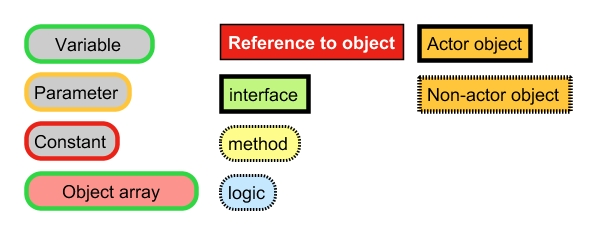
\includegraphics[width=0.75\columnwidth]{ChapterFramework/figures/Obj_key}%
%\includegraphics[width=0.85\columnwidth]{ChapterModels/Figures/hillclimbExcel}%
\caption{Key for model framework diagrams}%
\label{fig:frameworkKey}%
\end{figure}

%%%%%%%%%%%%%%%%%%%%%%%%%%%%%%%%%
Consider a person, labelled $a$, who is looking for a firm $f$ offering the best wage. Actors all have location, so let the distance between them be $af$. If people have to `commute' to their work place, the time taken to commute is zero sum with the time they can put into working. Here, a `commute' is taken to be twice $af$. The upper distance limit on whether a firm enters into $a$'s considerations has to be less than $a$'s one available day in total - half a day there, half back - otherwise there is no time left at all to contribute to production. So $f$ can only be a maximum of half a day away. If $c_{af}$ is the commute time between them then -

\[
c_{af}=2\cdot t_{af}\]

The set of potential employers for a person is thus immediately limited by commute distance. This set of potential employers is labelled as $PE_{a}=\{f_{n}...\}$ It can contain any number of firms within commute range. The set of firms is just  $F=\{f_{1},f_{2},...,f_{n}\}$ So, $p$ uses the following to populate $PE_{a}$:

\[
for\, each\, f_{n}\in F\]

\[
if(c_{af(n)}<1)\, then\, f_{n}\in PE_{a}\label{eq:circlerule}\]

Which translates as: unless the time it takes for $a$ to get to $f_{n}$ and back again (the commute distance) is more than one, add it to my set of potential employers. This guarantees there is time left for working, and $a$ can then use it to see if working is worthwhile. 

%This varies between model types, but what all models share is that people's wage will be proportional to the time they can contribute. In the simplest, the `wage' is a single good: the direct product of $a$'s contributed labour. 
So what is a `best wage?' If firms are paying in money, this is the maximum amount a person can get, having accounted for any commute loss. 

So $a$'s actual wage is:

\[
w_{a}=W_{f}\cdot l_{a}\]

This creates a new set: a list of wages from $PE_{a}$:

\[
Wagelist_{a} = 
\]

Whether paid in raw goods or money, what this means is that, for the set of potential employers, $PE_{a}$, there is always one objectively best wage, since distance cost has been accounted for. It also mean that, if wages are the same for all firms, the nearest firm offers the best wage.

So $a$ selects the one firm with the maximum wage and adds it to the Bundle:

$bestwage = max{}$

\cmt{blah! Do I really need to be going to these lengths just to say `select firm with best wage, accounting for commute costs?' Must be a more succinct way!}

%Depending on the model, people may be able to choose between working and backyard production. Backyard production is linear: if people are producing for themselves, time can be converted directly into goods. 
%In this case, $t$ is literally the budget: $u$ can be maximised with a budget of $x+y=t=1$. Space does not enter into this decision: by definition, backyard production means staying put.

%Consider a generic utility function with two goods: $u=f(x,y)$. The `budget' a person has to work with is, at base, one day or $t=1$. However, $t$ needs converting into goods before a utility value can be found. Depending on the model, matters are complicated because $t$ can be converted into either goods or money first - via a wage - and then to goods. But what about working?

%The most complicated set of steps a person will have to take involves earning a money wage and then seeking to buy goods with that wage. People know nothing about any firm's productivity. They only know the wages and goods prices they find, and their own utility function. So a person cannot know what quantity of goods they can get without first knowing a wage and goods prices. 

%%%%%%%%%%%%%%%

%The method used is a stochastic search: budget `slices' are randomly allotted to each good and then adjusted towards better mixes (see the code appendix and comments within the classes themselves for full details.) 
%To do this, the best wage is split into randomly sized `slices' of money and whatever quantity of goods that would buy is 
%that gets us. Or we don't if stock is out: we try to reallocate, until either all stock is gone or all money is gone. That seems easier explained in words than in anything else. Hmm.

\end{comment}